\section{Постановка задачи}
Цель работы --- исследовать влияние L1-, L2- и ElasticNet-регуляризации на линейные модели, обученные на данных и наборах признаков первой лабораторной работы.

Необходимо разделить данные на обучающую, валидационную и тестовую части, оценивать параметры нормировки только на обучении и реализовать регуляризацию средствами NumPy и Pandas. Свободный коэффициент не должен штрафоваться. Аналитическое обучение линейной регрессии следует заменить градиентным спуском.

Для каждого набора признаков требуется сравнить четыре режима при одинаковых начальных весах, разбиении, шаге обучения и числе итераций. Параметр регуляризации проверяется как минимум на трёх значениях; для ElasticNet дополнительно исследуются как минимум три соотношения L1 и L2. Параметры выбираются по валидации. Для выбранных конфигураций строятся четыре графика: MSE и $R^2$ на обучении и валидации в зависимости от итерации. На каждом графике должны присутствовать все четыре режима, а MSE рассчитывается без штрафа. Итоговое сравнение включает тестовые метрики, переобучение и изменение коэффициентов, в том числе появление нулевых значений.

\section{Данные и наборы признаков}
Решается задача прогнозирования индекса успеваемости \textit{Performance Index}. Используется набор Student Performance: 10\,000 строк, пять исходных признаков и целевая переменная. Пропущенных значений нет. После удаления 127 полностью совпадающих строк остаются 9\,873 наблюдения.

Как и в первой работе, полные повторы удаляются до разбиения. Это исключает попадание одинаковых строк в разные части выборки. При этом совпадение всех значений само по себе не доказывает, что строки описывают одного и того же учащегося.

\begin{table}[H]\centering
\caption{Сравниваемые наборы признаков}
\begin{tabularx}{\textwidth}{llX}\toprule
Модель & Размерность & Признаки\\\midrule
M1 & 1 & Hours Studied: часы учёбы.\\
M2 & 2 & Часы учёбы и Previous Scores: предыдущие баллы.\\
M3 & 5 & M2, Extracurricular Activities, Sleep Hours и Sample Question Papers Practiced.\\
M4 & 6 & M3 и произведение Hours Studied $\times$ Previous Scores.\\\bottomrule
\end{tabularx}\end{table}

Категория внеучебных занятий кодируется как Yes $=1$, No $=0$. Предусмотрено заполнение числовых пропусков медианой, категориальных --- модой обучающей части. Произведение строится после заполнения пропусков. Все признаки, включая бинарный и составной, стандартизуются:
\[
z_j=\frac{x_j-\mu_j}{s_j},\qquad
\mu_j=\frac{1}{n}\sum_{i=1}^{n}x_{ij},\qquad
s_j=\sqrt{\frac{1}{n}\sum_{i=1}^{n}(x_{ij}-\mu_j)^2}.
\]
При $s_j=0$ используется масштаб 1. Валидация и тест преобразуются с теми же обучающими параметрами. Целевая переменная не масштабируется, прогноз не ограничивается допустимым диапазоном оценок.

\clearpage
\section{Модель и алгоритм обучения}
Для стандартизованного вектора признаков $z_i\in\mathbb{R}^{p}$ прогноз равен
\[
\hat y_i=b+z_i^\mathsf{T}w.
\]
Минимизируется единая целевая функция
\begin{equation}
J(b,w)=\frac{1}{2n}\sum_{i=1}^{n}(b+z_i^\mathsf{T}w-y_i)^2
+\lambda\left(\alpha\sum_{j=1}^{p}|w_j|
+\frac{1-\alpha}{2}\sum_{j=1}^{p}w_j^2\right).
\end{equation}
Здесь $\lambda\geq0$ задаёт силу штрафа; $\alpha=1$ соответствует L1, $\alpha=0$ --- L2, а $0<\alpha<1$ --- ElasticNet. При $\lambda=0$ получается обычная линейная регрессия. Свободный коэффициент $b$ не входит ни в одну норму.

\subsection{Градиентный шаг и мягкое пороговое преобразование}
Для ошибки $e=Zw+b\mathbf{1}-y$ градиенты гладкой части имеют вид
\[
g_b=\frac{1}{n}\mathbf{1}^{\mathsf T}e,\qquad
g_w=\frac{1}{n}Z^{\mathsf T}e+\lambda(1-\alpha)w.
\]
В точке $w_j=0$ модуль не дифференцируем. Поэтому для L1-слагаемого применяется проксимальный вариант градиентного спуска:
\begin{align}
b^{(k+1)}&=b^{(k)}-\eta g_b,\\
u&=w^{(k)}-\eta g_w,\\
w_j^{(k+1)}&=\operatorname{sign}(u_j)
\max\bigl(|u_j|-\eta\lambda\alpha,0\bigr).
\end{align}
Мягкий порог позволяет получать точные нули. Для L2 и режима без штрафа порог равен нулю, поэтому алгоритм совпадает с обычным пакетным градиентным спуском. Значение $\lambda$ относится именно к функции (1); при другой нормировке MSE численные значения штрафа потребовали бы пересчёта.

\subsection{Порядок вычислений и проверка реализации}
Сначала вычисляются $A=X^{\mathsf T}X/n$ и $c=X^{\mathsf T}y/n$, где $X=[\mathbf{1},Z]$. На каждой итерации градиент квадратичной части равен $A\beta-c$, $\beta=(b,w)$. Это тот же полный градиент, но без повторного прохода по всем строкам. Затем добавляется L2-слагаемое и выполняется пороговый шаг только для весов признаков.

Итерация 0 соответствует нулевым параметрам. Обучение не останавливается досрочно: каждая конфигурация выполняет полное заданное число шагов. Используется консервативная проверка $\eta L\leq1$, где $L$ ограничивается максимальной абсолютной суммой строки матрицы $A$ плюс $\lambda(1-\alpha)$.

Проверки охватывают известное решение на ортогональных признаках для всех четырёх режимов, отсутствие штрафа на свободный коэффициент, эквивалентность при $\lambda=0$, соответствие истории прямому вычислению MSE, изоляцию предобработки, разбиение данных и воспроизводимость сохранённых прогнозов. Для итоговых моделей дополнительно проверены условия оптимальности с учётом субградиента L1.

\clearpage
\section{Протокол эксперимента и выбор параметров}
Сохранена тестовая часть первой работы: 1\,975 строк. Из оставшихся 7\,898 наблюдений выделены 5\,923 обучающих и 1\,975 валидационных. Для внешней перестановки используется seed 42, для внутренней --- seed 43. Индексы частей не пересекаются. Веса всех моделей изначально равны нулю, шаг $\eta=0{,}05$, число итераций $K=15\,000$.

Для каждого штрафа проверяются
\[
\lambda\in\{0{,}001;\;0{,}01;\;0{,}1;\;1;\;10\},
\]
а для ElasticNet дополнительно $\alpha\in\{0{,}2;\;0{,}5;\;0{,}8\}$. На модель приходится $1+5+5+15=26$ конфигураций, всего --- 104. Диапазон включает слабое воздействие и выраженное сжатие коэффициентов.

Внутри каждого семейства выбирается минимальная MSE на валидации после последней итерации. Тестовые значения вычисляются только для четырёх выбранных режимов каждой модели. Для сопоставимости кривых итоговые модели сохраняют обучение на 5\,923 строках: объединение обучения и валидации после выбора параметров не выполняется.

\begin{table}[H]\centering\small
\caption{Выбранные параметры и ошибки без добавления штрафа}
\begin{tabular}{llrrrr}
\toprule
Модель & Метод & $\lambda$ & $\alpha$ & MSE$_{train}$ & MSE$_{val}$ \\
\midrule
M1 & Без рег. & 0 & -- & 314.657468 & 320.163893 \\
M1 & L1 & 0.1 & -- & 314.667468 & 320.104663 \\
M1 & L2 & 0.01 & -- & 314.662675 & 320.119203 \\
M1 & ElasticNet & 0.1 & 0.5 & 314.813255 & 320.042860 \\
M2 & Без рег. & 0 & -- & 5.291334 & 5.020790 \\
M2 & L1 & 0.001 & -- & 5.291336 & 5.020888 \\
M2 & L2 & 0.001 & -- & 5.291699 & 5.022199 \\
M2 & ElasticNet & 0.001 & 0.8 & 5.291358 & 5.021100 \\
M3 & Без рег. & 0 & -- & 4.178081 & 4.087215 \\
M3 & L1 & 0.001 & -- & 4.178085 & 4.087225 \\
M3 & L2 & 0.001 & -- & 4.178446 & 4.088265 \\
M3 & ElasticNet & 0.001 & 0.8 & 4.178107 & 4.087383 \\
M4 & Без рег. & 0 & -- & 4.178048 & 4.087260 \\
M4 & L1 & 0.001 & -- & 4.178055 & 4.087289 \\
M4 & L2 & 0.001 & -- & 4.182082 & 4.092679 \\
M4 & ElasticNet & 0.001 & 0.8 & 4.178259 & 4.087786 \\
\bottomrule
\end{tabular}

\end{table}

Для M2--M4 лучший штраф внутри каждого семейства находится на нижней границе сетки. При сравнении всех режимов валидация предпочитает отсутствие регуляризации. Это означает, что положительный штраф в исследованном диапазоне не даёт выигрыша для этих моделей. Глобально минимальная валидационная MSE получена у M3 без штрафа; именно эта конфигурация выбирается как основная. Для M1 небольшое сжатие улучшает валидацию, однако изменение мало по сравнению с её высокой общей ошибкой.

\clearpage
\section{Влияние силы и состава штрафа}
\begin{figure}[H]\centering
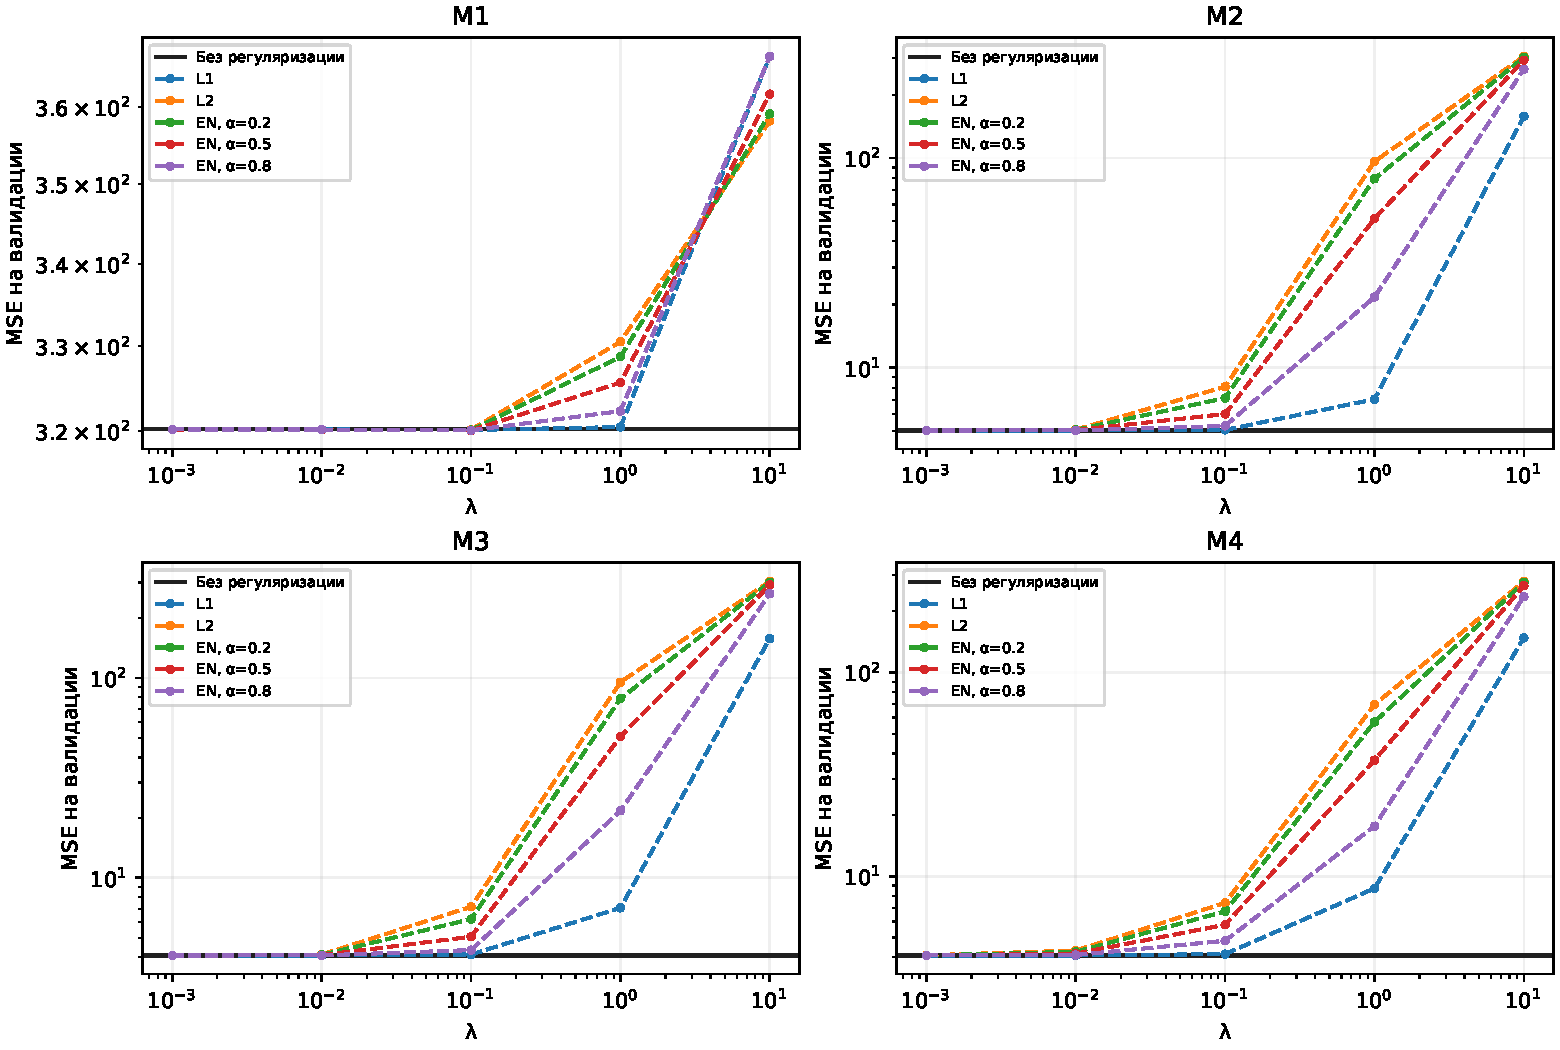
\includegraphics[width=\textwidth]{parameter_search.pdf}
\caption{Валидационная MSE в зависимости от $\lambda$. Обе оси логарифмические; EN обозначает ElasticNet. Горизонтальная линия показывает отсутствие штрафа.}
\end{figure}

Для M2--M4 увеличение штрафа повышает ошибку: смещение, вызванное сжатием информативных коэффициентов, становится существенным. При малых $\lambda$ различия между кривыми почти незаметны. Для ElasticNet больший вклад L1 даёт меньшую ошибку у M2--M4 в выбранной сетке; для M1 лучший результат достигается при $\alpha=0{,}5$ и $\lambda=0{,}1$. Следовательно, оптимальное соотношение зависит от набора признаков.

\begin{table}[H]\centering\small
\caption{Разреживание M3 при L1-регуляризации; свободный коэффициент исключён}
\begin{tabular}{rrrrr}
\toprule
$\lambda$ & MSE$_{val}$ & $\|w\|_1$ & $\|w\|_2$ & Нулей \\
\midrule
0.001 & 4.087225 & 26.657557 & 19.095360 & 0 \\
0.01 & 4.087737 & 26.613523 & 19.082996 & 0 \\
0.1 & 4.133985 & 26.173182 & 18.960035 & 0 \\
1 & 7.072813 & 22.978633 & 17.773383 & 3 \\
10 & 157.497739 & 7.541279 & 7.541279 & 4 \\
\bottomrule
\end{tabular}

\end{table}

При $\lambda=1$ в M3 обнуляются коэффициенты внеучебных занятий, сна и решённых вариантов: остаются часы учёбы и предыдущие баллы. При $\lambda=10$ остаются только предыдущие баллы. Таким образом, точное зануление реализовано, но для этих данных оно сопровождается ухудшением качества. Порог близости к нулю далее принят равным $|w_j|<0{,}01$ в стандартизованной шкале.

\clearpage
\section{Динамика обучения}
На каждом из четырёх графиков для каждой модели показаны все режимы с параметрами из таблицы 2. Для различения совпадающих кривых используются разные цвета и штрихи. По оси итераций применяется симметричная логарифмическая шкала с линейной областью до 10; нулевая итерация сохранена. MSE показана в логарифмической шкале, $R^2$ --- в линейной.

Для любой части выборки размера $m$ метрики вычисляются как
\[
\operatorname{MSE}=\frac{1}{m}\sum_{i=1}^{m}(y_i-\hat y_i)^2,\qquad
R^2=1-\frac{\sum_i(y_i-\hat y_i)^2}{\sum_i(y_i-\bar y)^2}.
\]
Среднее $\bar y$ берётся по той части, на которой оценивается метрика; оно используется только при оценке, а не для обучения. Штраф к MSE не прибавляется. Отрицательные начальные значения $R^2$ допустимы: нулевой прогноз хуже константы, равной среднему целевой переменной.

\subsection{Модель M1}
\begin{figure}[H]\centering
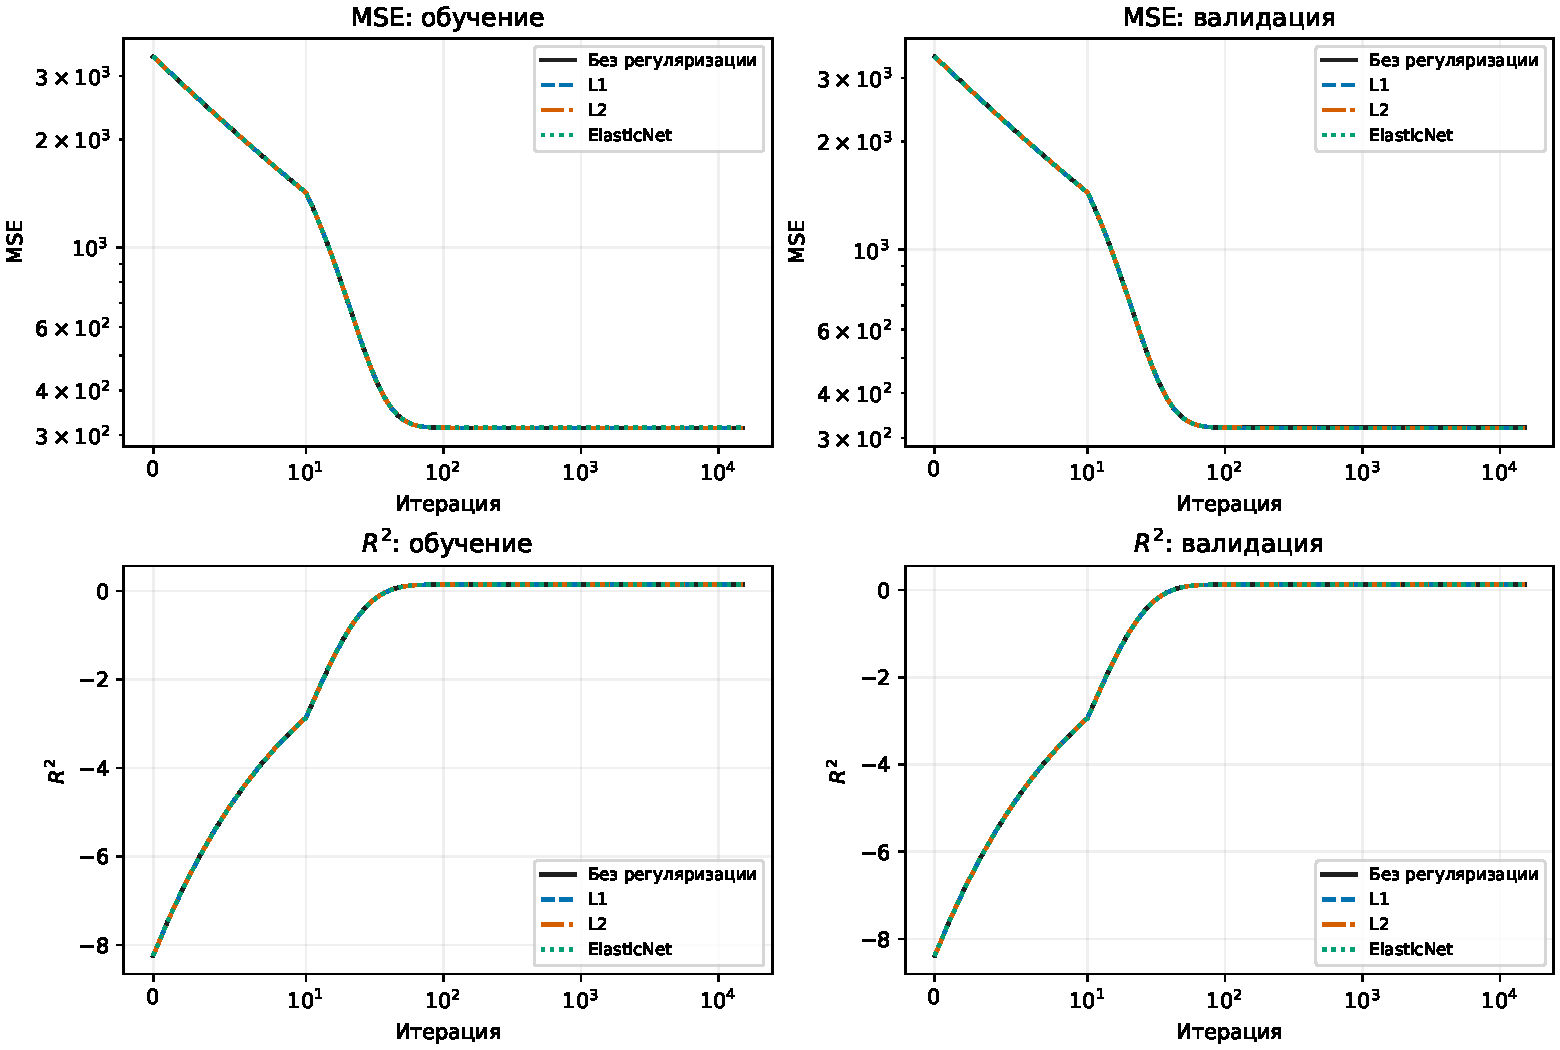
\includegraphics[width=\textwidth]{M1_curves.pdf}
\caption{M1: ошибки и качество на обучении и валидации.}
\end{figure}
Все режимы быстро выходят на плато. Низкое значение $R^2$ связано прежде всего с недостатком признаков: один признак не объясняет основную часть вариации целевой переменной. Регуляризация не устраняет такое недообучение. У ElasticNet валидационная MSE уменьшается с 320{,}164 до 320{,}043, однако тестовая MSE возрастает с 320{,}747 до 320{,}942.

\clearpage
\subsection{Модель M2}
\begin{figure}[H]\centering
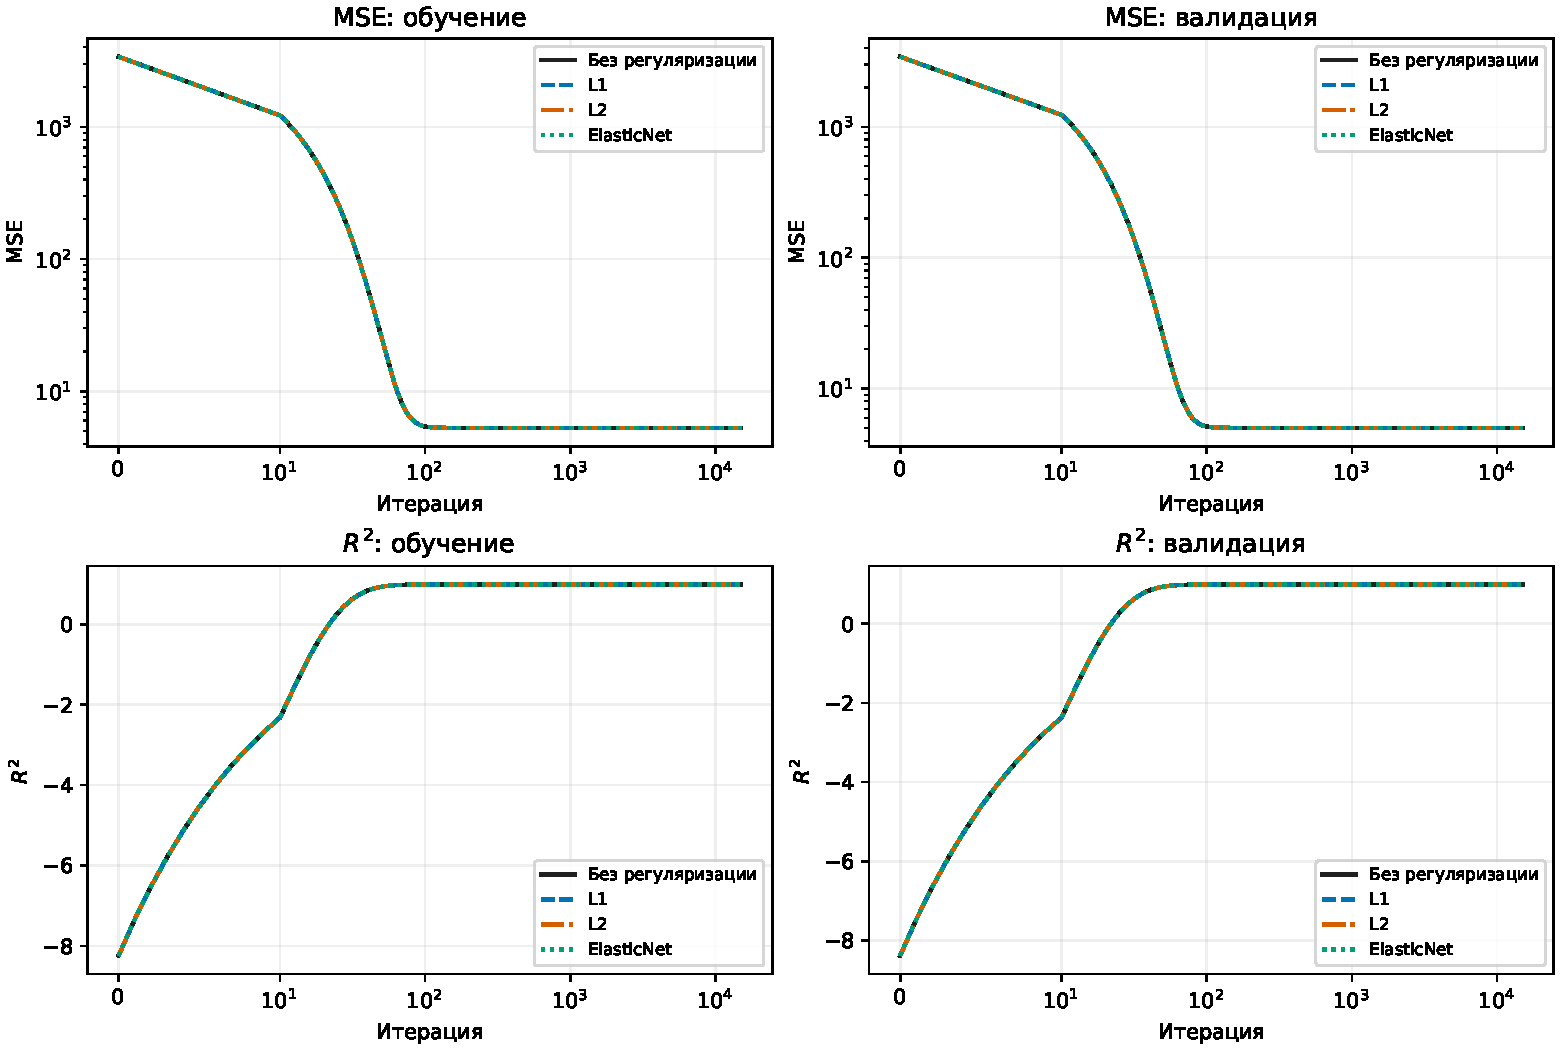
\includegraphics[width=\textwidth]{M2_curves.pdf}
\caption{M2: ошибки и качество на обучении и валидации.}
\end{figure}

Добавление предыдущих баллов резко снижает ошибку. Обучающая MSE без штрафа составляет 5{,}291334, валидационная --- 5{,}020790. При выбранных малых штрафах четыре траектории почти совпадают: влияние регуляризации существенно меньше эффекта добавленного признака.

Валидация предпочитает обычную линейную регрессию. Незначительно меньшая тестовая ошибка L2 не является основанием переопределять выбранную конфигурацию. Отличие тестового $R^2$ составляет лишь несколько миллионных и не подтверждает устойчивого преимущества метода.

Кривые не демонстрируют роста валидационной ошибки на поздних итерациях. Регуляризация в данном случае не решает явно наблюдаемую проблему переобучения: двух информативных признаков и доступного объёма обучения достаточно для устойчивой подгонки простой линейной модели.

\clearpage
\subsection{Модель M3}
\begin{figure}[H]\centering
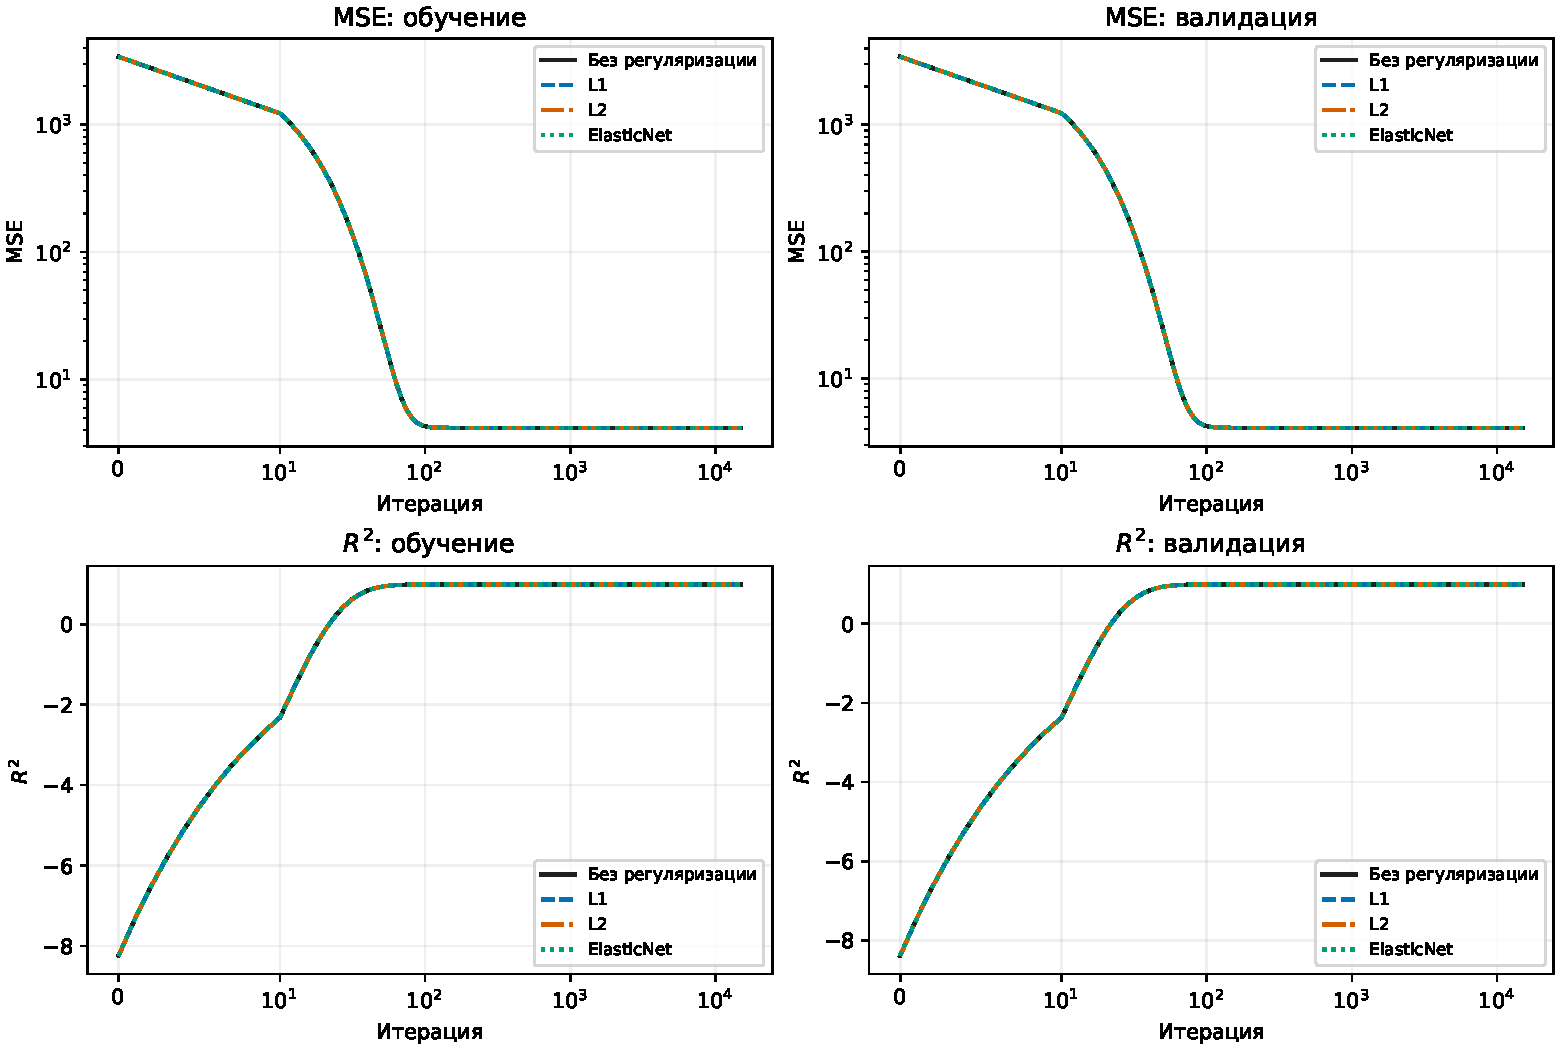
\includegraphics[width=\textwidth]{M3_curves.pdf}
\caption{M3: ошибки и качество на обучении и валидации.}
\end{figure}

Пять исходных признаков дают меньшую ошибку, чем M2. Без регуляризации обучающая MSE равна 4{,}178081, валидационная --- 4{,}087215, тестовая --- 4{,}262393. Значения на трёх частях близки; выраженного разрыва между обучением и проверкой не наблюдается.

Для L1, L2 и ElasticNet выбирается $\lambda=0{,}001$, для ElasticNet --- $\alpha=0{,}8$. При столь слабом штрафе кривые визуально почти совпадают. Это ожидаемое следствие малого изменения коэффициентов, а не отсутствие отдельных запусков.

На валидации M3 без штрафа лучше остальных исследованных конфигураций. Её тестовый $R^2=0{,}988621$. Тестовая MSE у L2 немного ниже, но разница около 0{,}000915, или 0{,}0215\%, слишком мала для вывода о надёжном выигрыше по одному разбиению.

\clearpage
\subsection{Модель M4}
\begin{figure}[H]\centering
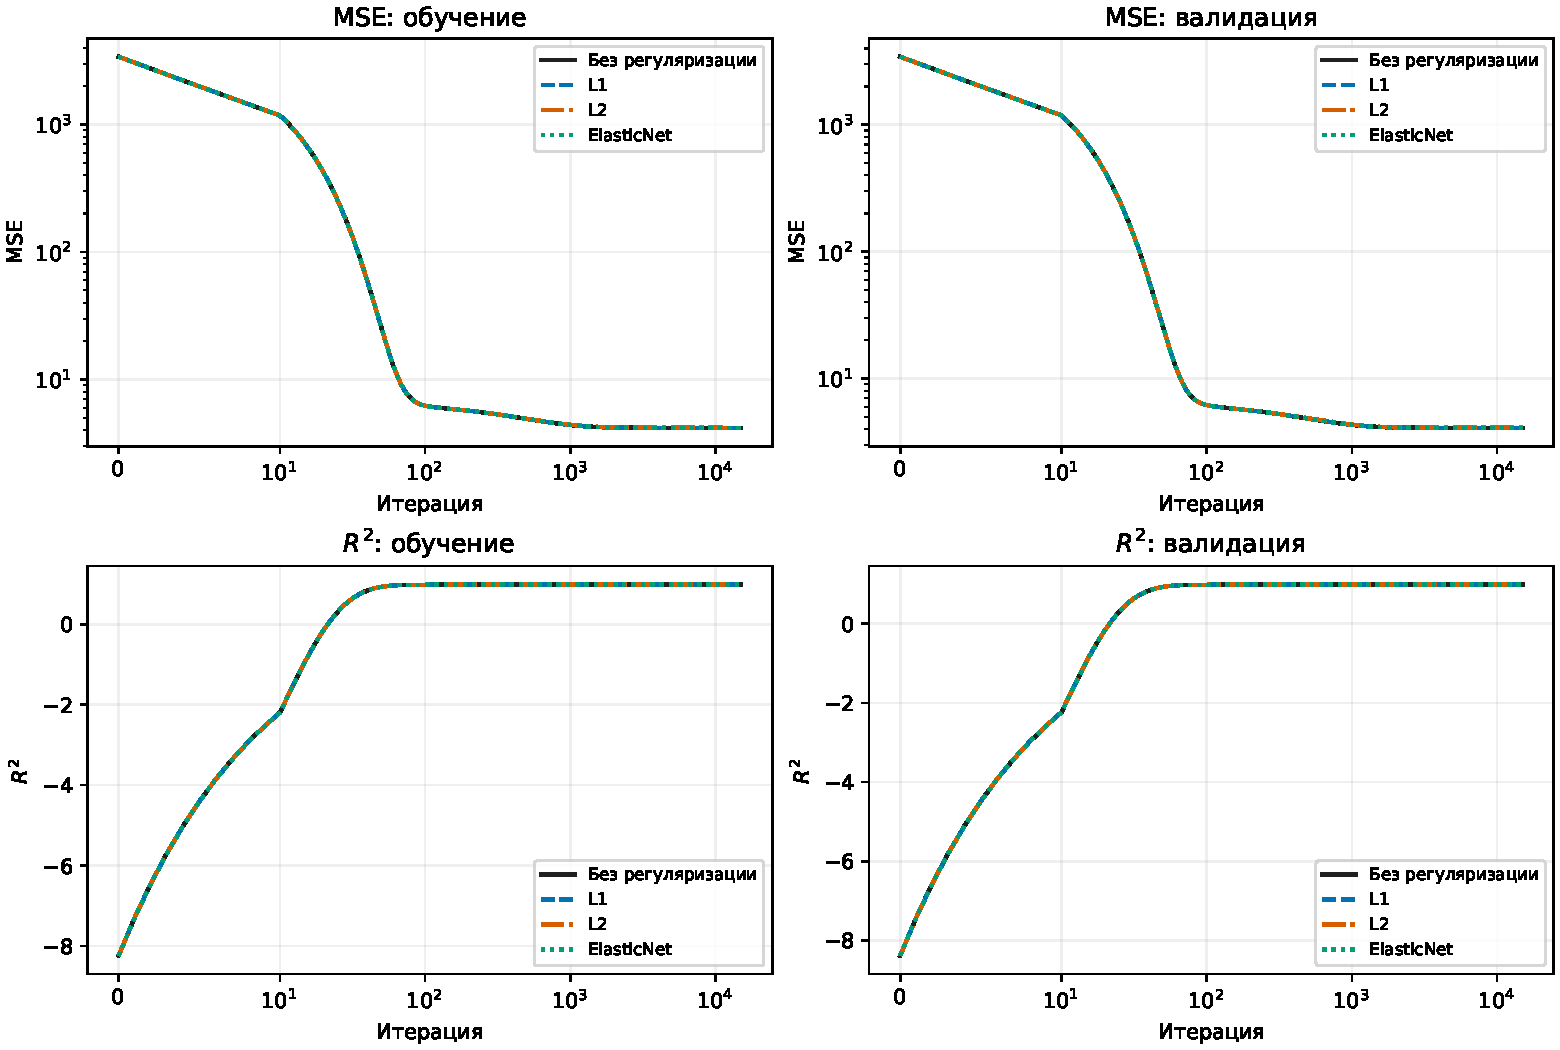
\includegraphics[width=\textwidth]{M4_curves.pdf}
\caption{M4: ошибки и качество на обучении и валидации.}
\end{figure}

Произведение часов учёбы и предыдущих баллов коррелирует с исходными признаками. Вследствие этого параметры перераспределяются между связанными столбцами, а сходимость идёт медленнее. Единые 15\,000 итераций позволяют довести все выбранные конфигурации до малой невязки условий оптимальности.

Добавление признака едва снижает обучающую MSE: с 4{,}178081 у M3 до 4{,}178048 у M4 без штрафа. Валидационная и тестовая ошибки при этом немного растут. Дополнительная сложность не даёт практически значимого улучшения.

L2 уменьшает общую евклидову норму весов, однако коэффициент произведения увеличивается за счёт уменьшения коэффициентов исходных признаков. Поэтому утверждение, что регуляризация обязательно уменьшает модуль каждого отдельного коэффициента, неверно при связанных признаках. Для выбранного L2 тестовая ошибка M4 составляет около 4{,}272144, что выше ошибки M3.

\clearpage
\section{Результаты на тестовом наборе}
После завершения выбора параметров оценены 16 итоговых моделей на одинаковых 1\,975 тестовых наблюдениях. Кроме обязательных MSE и $R^2$, приведены RMSE и MAE:
\[
\operatorname{RMSE}=\sqrt{\operatorname{MSE}},\qquad
\operatorname{MAE}=\frac{1}{m}\sum_{i=1}^{m}|y_i-\hat y_i|.
\]
\begin{table}[H]\centering\small
\caption{Общая таблица тестовых метрик}
\begin{tabular}{llrrrr}
\toprule
Модель & Метод & MSE & RMSE & MAE & $R^2$ \\
\midrule
M1 & Без рег. & 320.747102 & 17.909414 & 15.507152 & 0.143722 \\
M1 & L1 & 320.766775 & 17.909963 & 15.506227 & 0.143669 \\
M1 & L2 & 320.759280 & 17.909754 & 15.506399 & 0.143689 \\
M1 & ElasticNet & 320.941627 & 17.914844 & 15.506087 & 0.143202 \\
M2 & Без рег. & 5.314830 & 2.305391 & 1.827010 & 0.985811 \\
M2 & L1 & 5.314820 & 2.305389 & 1.827019 & 0.985811 \\
M2 & L2 & 5.314138 & 2.305241 & 1.827014 & 0.985813 \\
M2 & ElasticNet & 5.314632 & 2.305348 & 1.827015 & 0.985812 \\
M3 & Без рег. & 4.262393 & 2.064556 & 1.640506 & 0.988621 \\
M3 & L1 & 4.262333 & 2.064542 & 1.640512 & 0.988621 \\
M3 & L2 & 4.261478 & 2.064335 & 1.640716 & 0.988623 \\
M3 & ElasticNet & 4.262110 & 2.064488 & 1.640542 & 0.988622 \\
M4 & Без рег. & 4.262949 & 2.064691 & 1.640649 & 0.988619 \\
M4 & L1 & 4.263030 & 2.064711 & 1.640684 & 0.988619 \\
M4 & L2 & 4.272144 & 2.066917 & 1.643151 & 0.988595 \\
M4 & ElasticNet & 4.264262 & 2.065009 & 1.641105 & 0.988616 \\
\bottomrule
\end{tabular}

\end{table}

\subsection{Качество и переобучение}
Наибольший эффект даёт выбор информативных признаков: переход от M1 к M2 уменьшает MSE примерно с 321 до 5{,}3, а добавление остальных исходных признаков --- до 4{,}26. Различия между типами слабой регуляризации значительно меньше этих изменений.

Для M3 без штрафа разность тестовой и обучающей MSE составляет около 0{,}0843. M4 не улучшает обобщение по сравнению с M3, но столь малое изменение на одном разбиении нельзя считать доказательством серьёзного переобучения. У M1 высоки обе ошибки, что характерно для недостаточной выразительности набора признаков.

Минимальная наблюдаемая тестовая MSE в таблице принадлежит M3 с L2. Однако основная модель --- M3 без штрафа --- была выбрана по валидации до анализа теста. Разовый небольшой тестовый выигрыш не используется для повторного подбора параметров. Для оценки устойчивости различий потребовались бы повторные независимые разбиения или перекрёстная проверка.

\clearpage
\section{Изменение коэффициентов}
Ниже сравниваются веса стандартизованных признаков, поэтому их масштаб сопоставим. Свободный коэффициент для всех выбранных моделей равен среднему целевой переменной обучения: $b=55{,}042377$. Его совпадение обусловлено центрированием признаков и отсутствием штрафа на $b$.

\begin{table}[H]\centering\small
\caption{Стандартизованные коэффициенты M3}
\begin{tabular}{lrrrr}
\toprule
Признак & Без рег. & L1 & L2 & ElasticNet \\
\midrule
Часы учёбы & 7.391073 & 7.390088 & 7.383575 & 7.388784 \\
Предыдущие баллы & 17.577230 & 17.576244 & 17.559624 & 17.572918 \\
Внеучебные занятия & 0.293555 & 0.292559 & 0.293355 & 0.292719 \\
Часы сна & 0.825459 & 0.824453 & 0.824624 & 0.824487 \\
Решённые варианты & 0.575134 & 0.574213 & 0.575046 & 0.574380 \\
\bottomrule
\end{tabular}

\end{table}
\begin{table}[H]\centering\small
\caption{Стандартизованные коэффициенты M4}
\begin{tabular}{lrrrr}
\toprule
Признак & Без рег. & L1 & L2 & ElasticNet \\
\midrule
Часы учёбы & 7.368158 & 7.361718 & 7.117794 & 7.311333 \\
Предыдущие баллы & 17.566250 & 17.562651 & 17.432277 & 17.535807 \\
Внеучебные занятия & 0.293519 & 0.292514 & 0.292932 & 0.292596 \\
Часы сна & 0.825615 & 0.824645 & 0.826425 & 0.825012 \\
Решённые варианты & 0.575152 & 0.574236 & 0.575246 & 0.574440 \\
Произведение & 0.025982 & 0.032168 & 0.301662 & 0.087837 \\
\bottomrule
\end{tabular}

\end{table}

В выбранных по валидации конфигурациях точных нулей нет. Нет и коэффициентов с $|w_j|<0{,}01$. Это не противоречит свойствам L1: оптимальный по валидации штраф слишком мал для зануления данных весов. При более сильном штрафе нули появляются, как показано в таблице 3.

Коэффициент произведения у M4 без штрафа близок к 0{,}0260, а при L2 --- к 0{,}3017: вклады связанных признаков перераспределяются. В исходных единицах $\tilde w_j=w_j/s_j$, $\tilde b=b-\sum_j w_j\mu_j/s_j$. Поэтому исходный свободный коэффициент может различаться между режимами. Порог 0{,}01 применяется только к стандартизованным весам.

\section{Заключение}
Реализованы и проверены четыре режима регуляризации. Выполнены 104 конфигурации при одинаковых условиях оптимизации, построены 16 требуемых графиков. Предобработка и выбор параметров изолированы от тестового набора.

По валидации выбрана M3 без регуляризации: тестовая MSE равна 4{,}262393, $R^2=0{,}988621$. Слабые штрафы почти не меняют качество, а сильные увеличивают ошибку. L1 действительно создаёт разреженные решения, однако здесь удаление признаков ухудшает прогноз. Добавление произведения признаков не улучшает обобщение. Регуляризация управляет величиной и структурой весов, но её польза для качества должна подтверждаться валидацией и не является гарантированной.
